\documentclass[12pt]{report}
\usepackage[utf8]{inputenc}
\usepackage[russian]{babel}
%\usepackage[14pt]{extsizes}
\usepackage{listings}

% Для листинга кода:
\lstset{ %
language=python,                 % выбор языка для подсветки (здесь это С)
basicstyle=\small\sffamily, % размер и начертание шрифта для подсветки кода
numbers=left,               % где поставить нумерацию строк (слева\справа)
numberstyle=\tiny,           % размер шрифта для номеров строк
stepnumber=1,                   % размер шага между двумя номерами строк
numbersep=5pt,                % как далеко отстоят номера строк от подсвечиваемого кода
showspaces=false,            % показывать или нет пробелы специальными отступами
showstringspaces=false,      % показывать или нет пробелы в строках
showtabs=false,             % показывать или нет табуляцию в строках
frame=single,              % рисовать рамку вокруг кода
tabsize=2,                 % размер табуляции по умолчанию равен 2 пробелам
captionpos=t,              % позиция заголовка вверху [t] или внизу [b] 
breaklines=true,           % автоматически переносить строки (да\нет)
breakatwhitespace=false, % переносить строки только если есть пробел
escapeinside={\#*}{*)}   % если нужно добавить комментарии в коде
}

% Для измененных титулов глав:
\usepackage{titlesec, blindtext, color} % подключаем нужные пакеты
\definecolor{gray75}{gray}{0.75} % определяем цвет
\newcommand{\hsp}{\hspace{20pt}} % длина линии в 20pt
% titleformat определяет стиль
\titleformat{\chapter}[hang]{\Huge\bfseries}{\thechapter\hsp\textcolor{gray75}{|}\hsp}{0pt}{\Huge\bfseries}


% plot
\usepackage{pgfplots}
\usepackage{filecontents}
\usetikzlibrary{datavisualization}
\usetikzlibrary{datavisualization.formats.functions}

\begin{document}
 
%\def\chaptername{} % убирает "Глава"
\begin{titlepage}
	\centering
	{\scshape\LARGE МГТУ им. Баумана \par}
	\vspace{3cm}
	{\scshape\Large Лабораторная работа №2\par}
	\vspace{0.5cm}	
	{\scshape\Large По курсу: "Анализ алгоритмов"\par}
	\vspace{1.5cm}
	{\huge\bfseries Алгоритмы умножения матриц\par}
	\vspace{2cm}
	\Large Работу выполнил: студент группы ИУ7-53Б Наместник Анастасия\par
	\vspace{0.5cm}
	\LargeПреподаватели:  Волкова Л.Л., Строганов Ю.В.\par

	\vfill
	\large \textit {Москва, 2020} \par
\end{titlepage}

\tableofcontents

\newpage
\chapter*{Введение}
\addcontentsline{toc}{chapter}{Введение}

\textbf{            		Матрица} - прямоугольная таблица, заполненная числами. Важнейшие характеристики матрицы – число строк и число столбцов. Сами числа называют элементами матрицы и характеризуют их положением в матрице, задавая номер строки и номер столбца и записывая их в виде двойного индекса, причем вначале записывают номер строки, а затем столбца. \\

Пусть есть два конечных множества.

\begin{enumerate}
	\item Номера строк: M = {1, 2,..., n}.
	\item Номера столбцов: N =  {1, 2,..., m}, где n и m - натуральные числа.
\end{enumerate}
Назовем матрицей A  размерностью m x n (n - строк, m - столбцов) с элементами из некоторого кольца или поля K  отображение вида A:N x M -> K. Матрица записывается как (формула \ref{eq:ref1}).

\begin{equation}
	A = \left(
	\begin{array}{cccc}
			a_{11} & a_{12} & \ldots & a_{1m} \\
			a_{21} & a_{22} & \ldots & a_{2m} \\
			\vdots & \vdots & \ddots & \vdots \\
			a_{n1} & a_{n2} & \ldots & a_{nm}
		\end{array}
	\right)
	\label{eq:ref1}
\end{equation}

Простейшими действиями с матрицами являются следующие операции.

\begin{enumerate}
  	\item Умножение матрицы на число. Для этого необходимо умножить каждый элемент матрицы на данное число.
	\item Сложение матриц. Складывать можно только матрицы одинакового размера, то есть имеющие одинаковое число строк и одинаковое число столбцов. При сложении матриц соответствующие их элементы складываются.
	\item Добавить оптимизации к алгоритму Винограда.
	\item Транспонирование матрицы. При транспонировании у матрицы строки становятся столбцами и наоборот.
\end{enumerate}

	Целью данной лабораторной работы является изучение, реализация и сравнительный анализ алгоритмов
стандартного алгоритма умножения матриц, алгоритма Винограда и алгоритма с оптимизациями. 

В данной лабораторной работе требуется решить четыре задачи.
\begin{enumerate}
  	\item Изучить и программно реализовать стандартный алгоритм умножения матриц.
	\item Изучить и программно реализовать алгоритм Винограда умножения матриц.
	\item Добавить оптимизации к алгоритму Винограда.
	\item Сделать сравнительный анализ по затрачиваемым ресурсам (времени) компьютера на реализацию каждого рассмотренного алгоритма.
\end{enumerate}


\chapter{Аналитическая часть}
\textit{Произведение матриц} AB состоит из всех возможных комбинаций скалярных произведений 
вектор-строк матрицы A и вектор-столбцов матрицы B (рис. \ref{fg:ref2}).

\begin{figure}[ht!]
	\centering{
		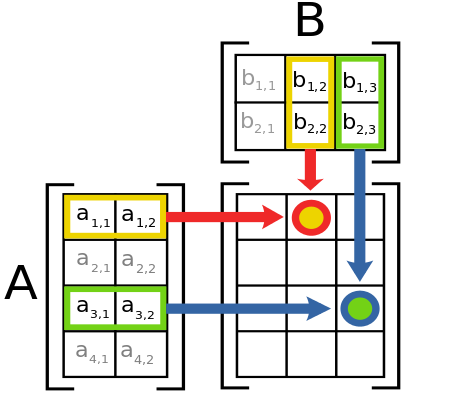
\includegraphics[width=0.5\textwidth]{pics/matrix_mult.png}
		\caption{Произведение матриц}
		\label{fg:ref2}}
\end{figure}

Операция умножения двух матриц выполнима только в том случае, если число столбцов в первой матрице равно числу строк во второй.

\section{Стандартный алгоритм умножения матриц}

Допустим имеется матрицы A (формула \ref{eq:ref1}) и B (формула \ref{eq:ref2})

\begin{equation}
	B = \left(
	\begin{array}{cccc}
			b_{11} & b_{12} & \ldots & b_{1m} \\
			b_{21} & b_{22} & \ldots & b_{2m} \\
			\vdots & \vdots & \ddots & \vdots \\
			b_{n1} & b_{n2} & \ldots & b_{nm}
		\end{array}
	\right)
	\label{eq:ref2}
\end{equation}

Матрица C = AB будет размерностью $l \times n$, 
где матрица A размерностью $l \times m$, а матрица B $m \times n$
Тогда каждый элемент матрицы C выражается формулой (\ref{eq:ref3})

\begin{equation}
	\begin{array}{cc}
		c_{ij} = \sum\limits_{r=1}^m a_{ir}b_{ri} & (i=1,2,\dots l; j=1,2,\dots n)
	\end{array}
	\label{eq:ref3}
\end{equation}

\section{Умножение матриц по Винограду}

Каждый элемент в матрице C, которая является результатом умножения двух матриц,
представляет собой скалярное произведение соответствующих строки и столбца исходных матриц. 
В алгоритме умножение матриц по Винограду предложено сделать предварительную обработку,
позволяющую часть работы выполнить заранее.

Рассмотрим два вектора V (формула \ref{eq:ref4}) и W (формула \ref{eq:ref5}).

\begin{equation}
	V = (v_1, v_2, v_3, v_4)
	\label{eq:ref4}
\end{equation}

\begin{equation}
	W = (w_1, w_2, w_3, w_4)
	\label{eq:ref5}
\end{equation}

Их скалярное произведение равно  \ref{eq:ref6}.

\begin{equation}
	V * W = v_1w_1 + v_2w_2 + v_3w_3 + v_4w_4
	\label{eq:ref6}
\end{equation}

Равенство \ref{eq:ref6} можно записать в виде \ref{eq:ref7}.

\begin{equation}
	\begin{array}{l}
		V * W = (v_1 + w_2)(v_2 + w_1) + (v_3 + w_4)(v_4 + w_3) - \\
		\quad \quad \quad v_1v_2 - v_3v_4 - w_1w_2 - w_3w_4
	\end{array}
	\label{eq:ref7}
\end{equation}

Выражение в правой части равенства \ref{eq:ref7} допускает предварительную обработку:
его части можно вычислить заранее и запомнить для каждой строки первой матрицы и для каждого столбца второй. На практике это означает,
что над предварительно обработанными элементами нам придется выполнять лишь первые два умножения и последующие пять сложений, а
также дополнительно два сложения. В случае нечетной общей размерности к каждому элементу результирующей матрицы следует добавить произведение элементов первой и второй матрицы, где каждый j-ый элемент первой матрицы и каждый i-ый элемент второй матрицы будут равны количеству столбцов первой матрицы.
Оптимизированный алгоритм Винограда умножения матриц допускает следующие модификации.

\begin{enumerate}
	\item Использование буфера вместо неоднократного обращения к ячейке памяти.
	\item Использование битовых (логических) операций.
\end{enumerate}


\section{Вывод}

Были рассмотрены основные теоретические сведения о различных способах реализации произведения матриц, которые в дальнейшем потребуются при разработке программного продукта.  

\chapter{Конструкторская часть}

\section{Схемы алгоритмов}

На рисунке \ref{fg:ref8} представлена схема стандартного алгоритма умножения матриц.

\begin{figure}[ht!]
	\centering{
		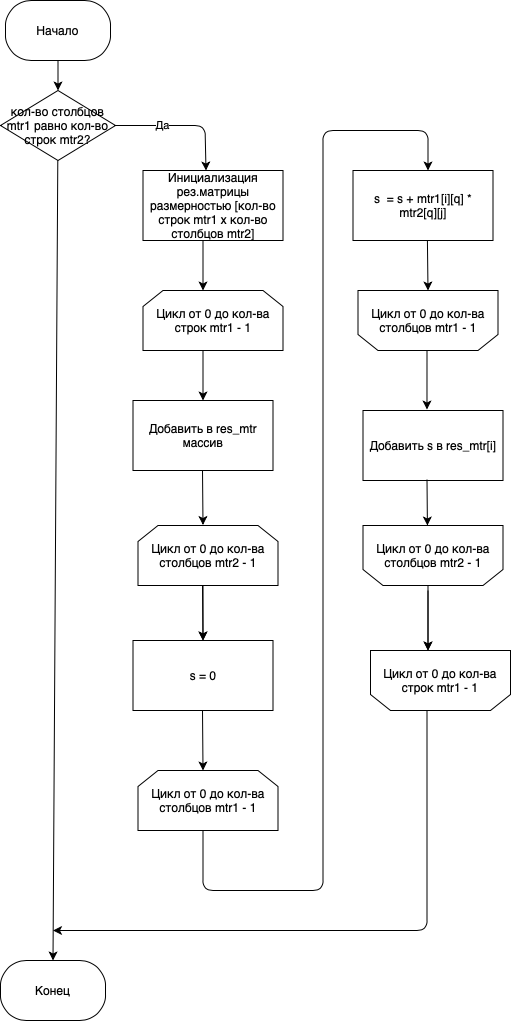
\includegraphics[scale=0.6]{schema/StandMtr.png}
		\caption{Схема алгоритма стандартного умножения матриц}
		\label{fg:ref8}}
\end{figure}

На рисунках \ref{fg:ref9} -\ref{fg:ref10} представлена схема алгоритма Винограда умножения матриц.

\begin{figure}[ht!]
	\centering{
		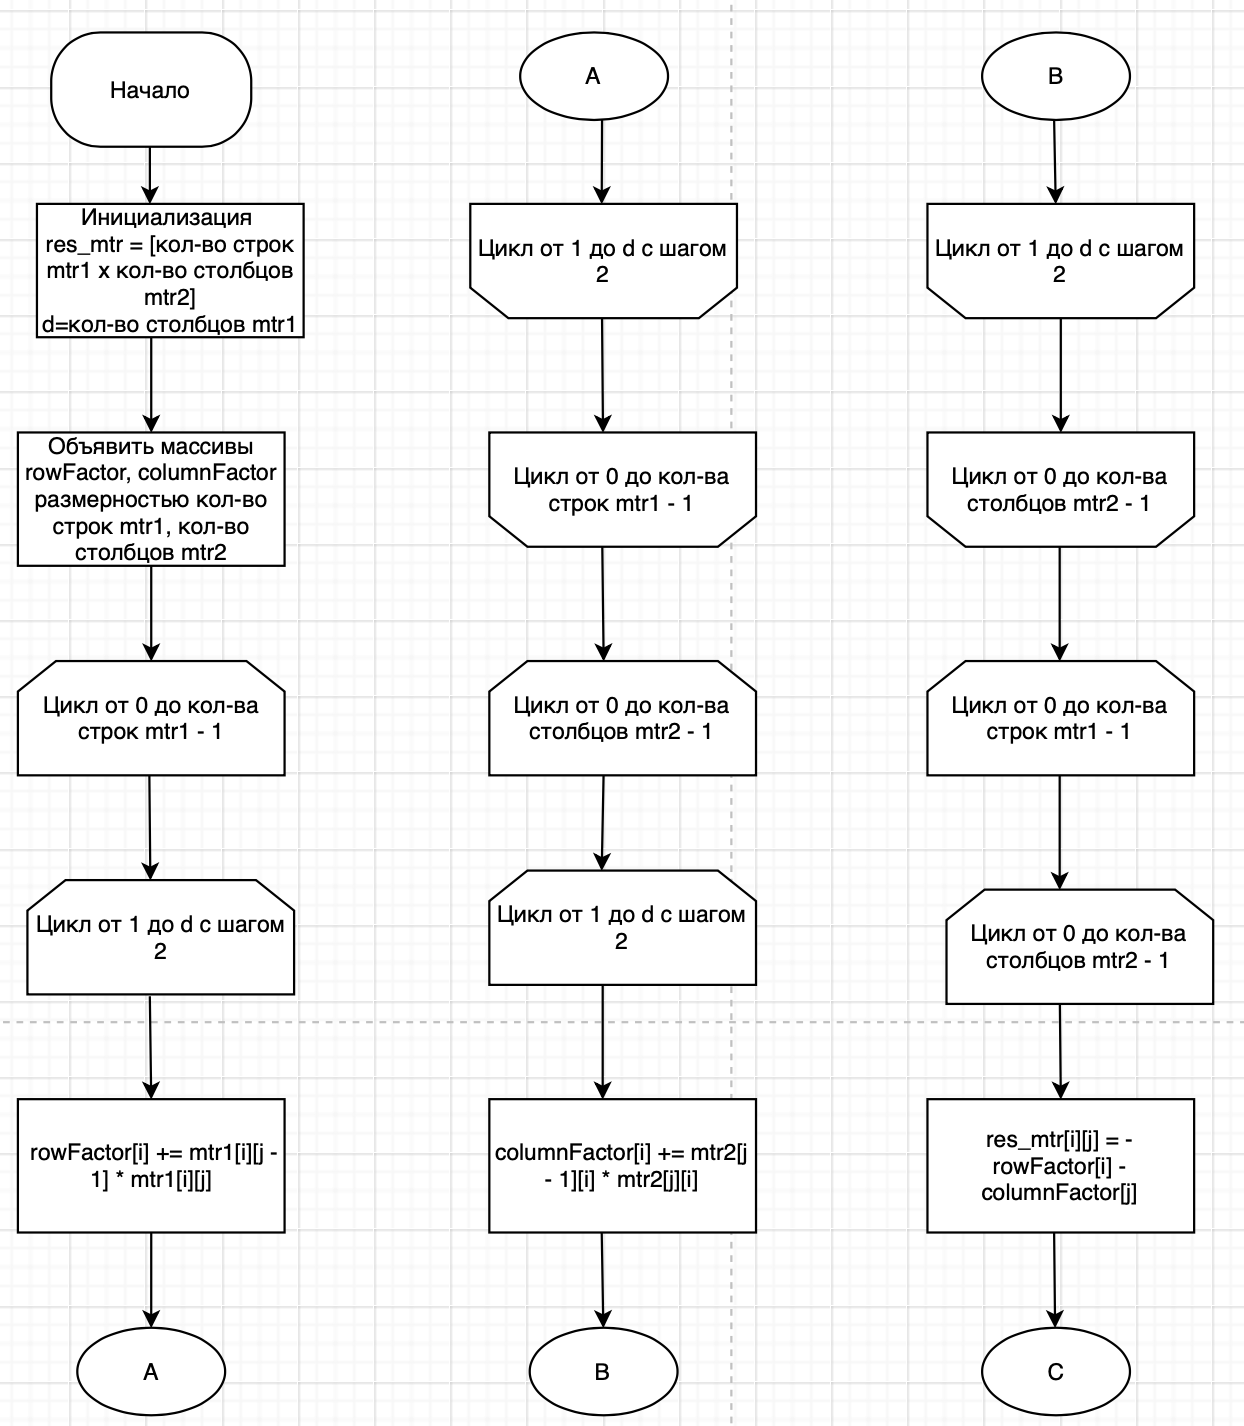
\includegraphics[scale=0.8]{schema/Win1.png}
		\caption{Схема алгоритма Винограда умножения матриц (начало)}
		\label{fg:ref9}}
\end{figure}

\begin{figure}[ht!]
	\centering{
		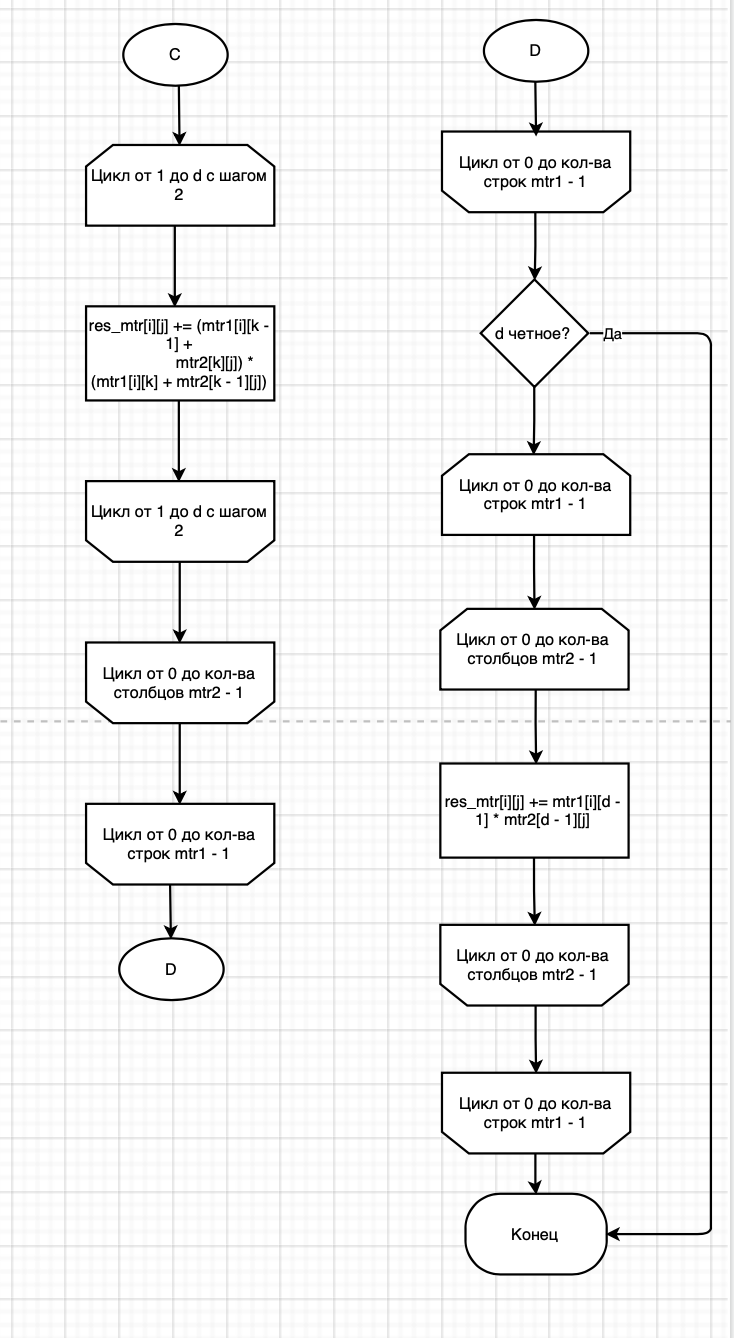
\includegraphics[scale = 0.8]{schema/Win2.png}
		\caption{Схема алгоритма Винограда умножения матриц (продолжение)}
		\label{fg:ref10}}
\end{figure}

 На рисунках \ref{fg:ref11}-\ref{fg:ref12} представлена схема оптимизированного алгоритма Винограда умножения матриц.

\begin{figure}[ht!]
	\centering{
		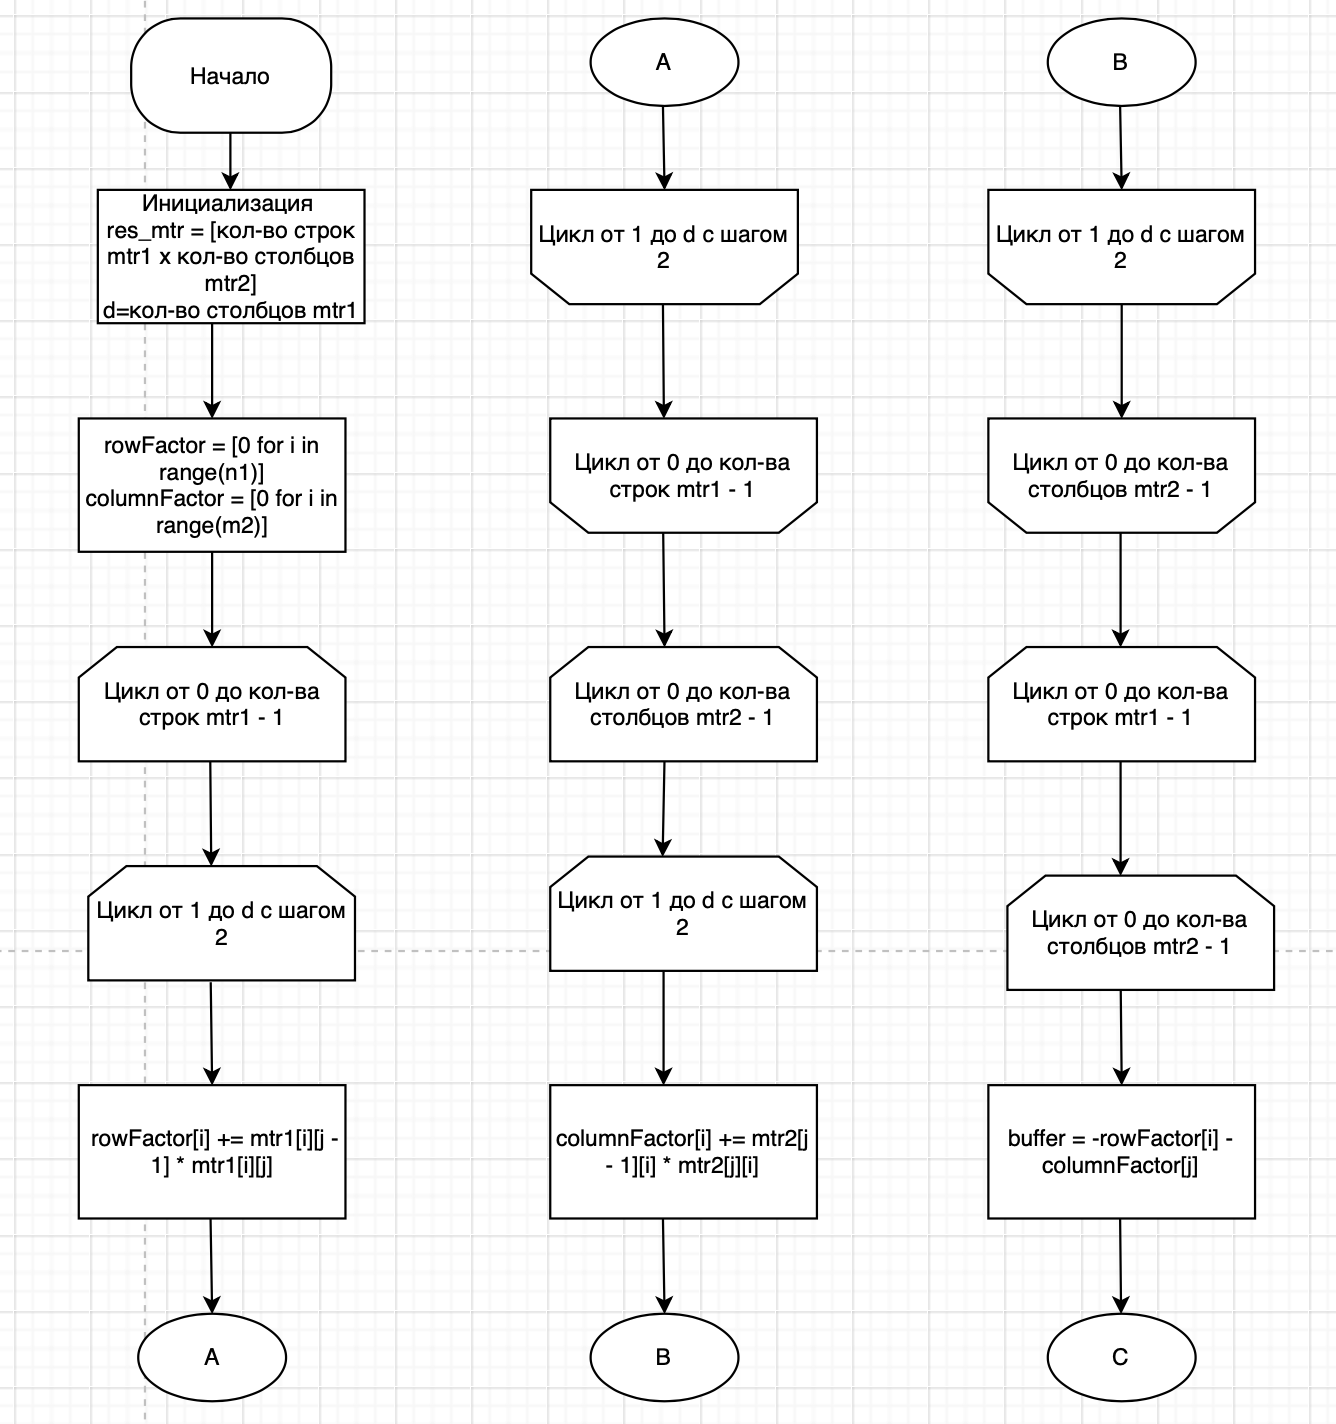
\includegraphics[scale=0.8]{schema/WinOpt1.png}
		\caption{Схема алгоритма Винограда умножения матриц с оптимизациями (начало)}
		\label{fg:ref11}}
\end{figure}

\begin{figure}[ht!]
	\centering{
		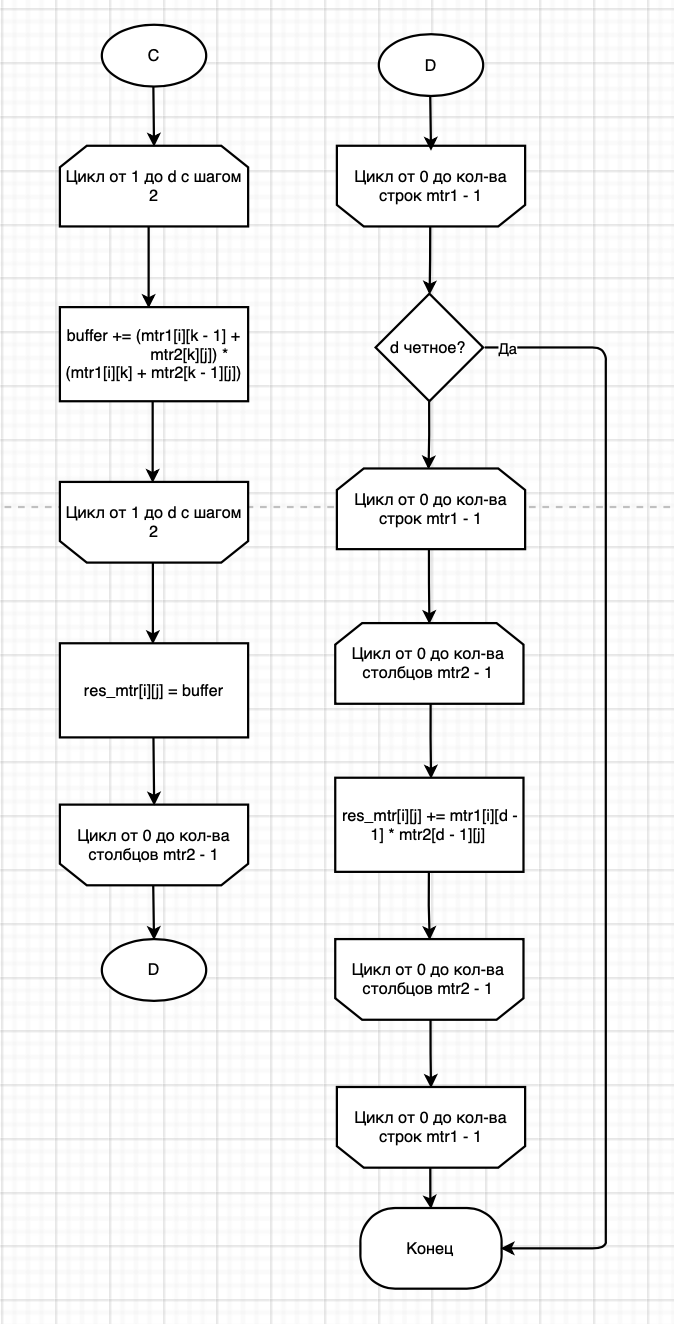
\includegraphics[scale = 0.8]{schema/WinOpt2.png}
		\caption{Схема алгоритма Винограда умножения матриц с оптимизациями (продолжение)}
		\label{fg:ref12}}
\end{figure}


\section{Вывод}
В данном разделе были рассмотрены схемы трех алгоритмов: стандартного алгоритма умножения матриц, алгоритма Винограда умножения матриц и алгоритма Винограда умножения матриц с оптимизациями. Из полученных данных можно отметить, что объем кода растет от стандартного алгоритма к оптимизированному алгоритму Винограда, что объясняется использованием дополнительных переменных и структур данных в алгоритме Винограда умножения матриц.

\chapter{Технологическая часть}
\section{Выбор языка программирования}
В данной лабораторной работе использовался язык программирования - python (3.8.3) \cite{bib1} в целях упрощения работы со структурами и визуализацией данных сравнительных анализов, а также из-за наличия опыта работы с данным языком программирования. В качестве интегрированной среды разработки использовался интерпретатор python - IDLE  \cite{bib2}. Для замеров процедурного времени использовалась функция process\_time() библиотеки time \cite{bib3}.  Для генерации матрицы использовалась функция randint() модуля random \cite{bib4}.

\section{Сведения о модулях программы}
Программа состоит из следующих модулей:
\begin{itemize}
	\item matrix.py - главный файл программы;
	\item time\_test.py - файл с замерами временнных характеристик.
\end{itemize}

\begin{lstlisting}[label=some-code,caption=Подпрограмма стандартного умножения матриц]
def StandMultMatrix(mtr1, mtr2, n1, m1, n2, m2):
    if m1 != n2:
        return False
    res_mtr = [np.full(m2, 0) for i in range(n1)]
    for i in range(n1):
        for j in range(m2):
            for q in range(m1):
                res_mtr[i][j] = res_mtr[i][j] + mtr1[i][q] * mtr2[q][j]
    return res_mtr

\end{lstlisting}

\begin{lstlisting}[label=some-code,caption=Подпрограмма алгоритма Винограда]
def WinogradMult(mtr1, mtr2, n1, m1, n2, m2):
    if m1 != n2:
        return False
    res_mtr = [np.full(m2, 0) for i in range(n1)]
    d = m1

    rowFactor = np.full(n1, 0)
    for i in range(n1):
        for j in range(1, d, 2):
            rowFactor[i] += mtr1[i][j - 1] * mtr1[i][j]

    columnFactor = np.full(m2, 0)
    for i in range(m2):
        for j in range(1, d, 2):
            columnFactor[i] += mtr2[j - 1][i] * mtr2[j][i]

    for i in range(n1):
        for j in range(m2):
            res_mtr[i][j] = -rowFactor[i] - columnFactor[j]
            for k in range(1, d, 2):
                res_mtr[i][j] += (mtr1[i][k - 1] +
                mtr2[k][j]) * (mtr1[i][k] + mtr2[k - 1][j])
    if d % 1:
        for i in range(n1):
            for j in range(m2):
                res_mtr[i][j] += mtr1[i][d - 1] * mtr2[d - 1][j]

    return res_mtr\end{lstlisting}

\begin{lstlisting}[label=some-code,caption=Подпрограмма алгоритма Винограда с оптимизациями]
def WinogradOptimization(mtr1, mtr2, n1, m1, n2, m2):
    if m1 != n2:
        return False
    res_mtr = [np.full(m2, 0) for i in range(n1)]
    d = m1
    
    #Optimization: stop using numpy methods
    rowFactor = [0 for i in range(n1)]
    for i in range(n1):
        for j in range(1, d, 2):
            rowFactor[i] += mtr1[i][j - 1] * mtr1[i][j]

    columnFactor = [0 for i in range(m2)]
    for i in range(m2):
        for j in range(1, d, 2):
            columnFactor[i] += mtr2[j - 1][i] * mtr2[j][i]

    #Optimization: buffer (stop frequent memory cell access request)
    for i in range(n1):
        for j in range(m2):
            buffer = -rowFactor[i] - columnFactor[j]
            for k in range(1, d, 2):
                buffer += (mtr1[i][k - 1] +
                mtr2[k][j]) * (mtr1[i][k] + mtr2[k - 1][j])
            res_mtr[i][j] = buffer
    #Optimization: bit operation & (and) instead of %
    if d & 1:
        for i in range(n1):
            for j in range(m2):
                res_mtr[i][j] += mtr1[i][d - 1] * mtr2[d - 1][j]

    return res_mtr
\end{lstlisting}

\begin{lstlisting}[label=some-code,caption=Подпрограмма создания матрицы]
def CreateMatrix(n, m):
    return [[int(j) for j in input().split()] for i in range(n)]
\end{lstlisting}

\begin{lstlisting}[label=some-code,caption=Подпрограмма создания матрицы с использованием функции randint модуля random  \cite{bib4}]
def CreateMatrixRandom(n, m):
    return [[randint(0, 100) for j in range(m)] for i in range(n)]\end{lstlisting}

\section{Тесты}

В данном разделе будет представлена таблица с тестами (таблица \ref{table:ref13})
\begin{table}[ht]
	\centering
	\caption{Сравнительная таблица времени выполнения всех алгоритмов при четной длине матицы}
	\begin{tabular}{|c c c|}
		\hline
		Матрица 1 & Матрица 2 &  Результат \\ [0.5ex] 
 		\hline\hline
		2 3 & 3 2 & Верный\\
 		\hline
 		1 5 & 5 1 & Верный\\
		\hline
		5 1 & 1 05 & Верный\\
 		\hline
 		 5 5 & 5 5 & Верный\\
 		\hline
		4 5 & 3 5 & Сообщение об ошибке\\
		\hline
	\end{tabular}
	\label{table:ref13}
\end{table} 

Примечание: в сообщении об ошибке указано, что количество строк Матрица1 не совпадает с количеством столбцов Матрица2.


\section{Вывод}
В технологической части были представлены модули программы, листинги кода и тестов к программе, а также обусловлен выбор языка программирования и приведены использовавшиеся в ходе работы инструменты.


\chapter{Исследовательская часть}

\section{Результат замеров времени выполнения всех алгоритмов} 

Сравним временные показатели работы каждого из рассматриваемых четырех алгоритмов при длине квадратной матрицы от 20 до 100 чисел. Для этого установим количество итераций (повторений вызова процедуры) iter и воспользуемся библиотекой time для замера времени выполнения каждого алгоритма по iter раз. Возьмем iter = 100, а размерность квадратных матриц равной [10, 20, 30, 40, 50, 60, 70, 80, 90, 100]. Время выполнения алгоритмов произведения матриц довольно мало, поэтому, чтобы оценить его, следует взять среднее арифметическое от времени, за которое процедура отработает установленные iter раз. 

На рисунке \ref{fg:ref14} показана работа алгоритмов с матрицами с четным количеством столбцов первой матрицы.

\begin{figure}[ht!]
	\centering{
		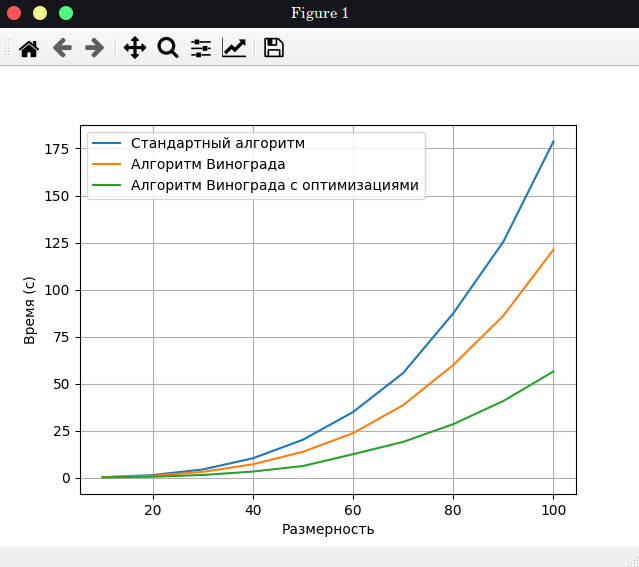
\includegraphics[width=0.6\textwidth]{pics/Time.png}
		\caption{Сравнение времени выполнения алгоритмов} 
		\label{fg:ref14}}
\end{figure}

На рисунке \ref{fg:ref15} показана работа алгоритмов с матрицами с нечетным количеством столбцов первой матрицы.

\begin{figure}[ht!]
	\centering{
		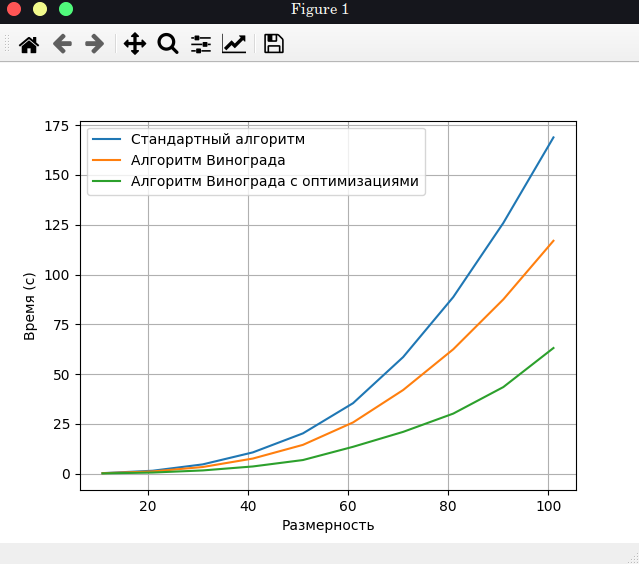
\includegraphics[width=0.8\textwidth]{pics/Time1.png}
		\caption{Временные характеристики на нечетных размерах матриц}
		\label{fg:ref15}}
\end{figure}

\par

В качестве примера на рисунке \ref{table:ref16} приведена таблица, представляющая временные характеристики всех алгоритмов при размере квадратной матрицы от 20 до 100 чисел.
\begin{table}[ht]
	\centering
	\caption{Сравнительная таблица времени выполнения (сек.) всех алгоритмов при четной длине матицы}
	\begin{tabular}{|c c c c|}
		\hline
		Разм. матриц & Станд. & Виноград & Виноград(опт)  \\ [0.5ex] 
 		\hline\hline
		20 & 0.0000360 & 0.0000345 & 0.0000235\\
 		\hline
 		30 & 0.0000751 & 0.0000617 & 0.0000386\\
 		\hline
 		40 & 0.0001221 & 0.0000986 & 0.0000576\\
 		\hline
		50 & 0.0001841 & 0.0001462 & 0.0000837\\
		\hline
		60 & 0.0002648 & 0.0001988 & 0.0001119\\
		\hline
		70 & 0.0003507 & 0.0002656 & 0.0001464\\
		\hline
		80 & 0.0004629 & 0.0003613 & 0.0001824\\
		\hline
		90 & 0.0005592 & 0.0004178 & 0.0002259\\
		\hline
		100 & 0.0007043 & 0.0005084 & 0.0002661\\
		\hline
	\end{tabular}
	\label{table:ref16}
\end{table} 

\section{Сравнительный анализ алгоритмов}

Введем модель вычислений трудоемкости алгоритма.
Пусть трудоемкость 1 у следующих базовых операций: +, -, *, /, =, ==, !=, <, <=, >, >=. Трудоемкость цикла: f цикла = f иниц + f сравн + N итер(f тела +
fинкрем + fсравн ).Трудоемкость условного перехода 1.

Стандартная реализация алгоритма не эффективна по времени, так как
обладает трудоемкостью 13N1M2M1+ 4N1M2+ 4N1 + 2.
Оценка трудоемкости данного алгоритма составляет 13N1M2M1. 
По памяти в стандартном алгоритме умножения матриц требуется m*n памяти под результат.

Теперь рассмотрим алгоритм Винограда умножения матриц. 
Реализация алгоритма Винограда обла­дает трудоемкостью 13M1M2 + 7M2 + ${15\over{2}}$ N1M1 + 7N1 + 13 N1M1M2 + 12N1M2 + 4N1 + 8 + (2, если M1 четное, 15N1M2 + 4N1 + 2, иначе).
Оценка трудоемкости данного алгоритма составляет 13N1M2M1 .
В алгоритме Винограда умножения матриц требуется дополнительно m+n памяти под результат.

Трудоемкость оптимизированного алгоритма Винограда с с учетом таких оптимизаций, как использование буфера и побитовой операции, будет примерно равна 9N1M1M2.



\section{Вывод}

В данном разделе было произведено сравнение количества затраченного вре­мени вышеизложенных алгоритмов.
Самым быстрым оказался оптимизированный алгоритм Винограда.
При этом в алгоритме Винограда умножения матриц требуется дополнительно m+n памяти под результат.

\chapter*{Заключение}
\addcontentsline{toc}{chapter}{Заключение}
В ходе лабораторной работы были реализованы и проанализированы алгоритм стандартного умножения матриц, алгоритм умножения матриц Винограда и алгоритм умножения матриц Винограда с оптимизациями. Было установлено, что благодаря предварительной обработки каждой строки первой матрицы и каждого столбца второй матрицы, результат которой сохранялся в двух дополнительных структурах данных - массивах, алгоритм умножения матриц Винограда значительно экономит время работы программы в сравнении со стандартным алгоритмом. Дополнительные оптимизации этого алгоритма позволили сделать его работу еще более эффективной по времени.

В рамках выполнения работы решены следующие задачи.

\begin{enumerate}
	\item Изучен и программно реализован стандартный алгоритм умножения матриц.
	\item Изучен и программно реализован алгоритм Винограда умножения матриц.
	\item Добавлены оптимизации к алгоритму Винограда.
	\item Сделан сравнительный анализ по затрачиваемым ресурсам (времени) компьютера на реализацию каждого рассмотренного алгоритма.

\end{enumerate}

\bibliographystyle{gost780u}
\bibliography{books}



\end{document}